\section{Graphenklassifikation} \label{sec:classification_theory}

Die Graphenklassifikation ist eine Aufgabe, über welche Graphen einer oder mehreren Klassen zugewiesen werden.
Der Anfang der Graphenklassifikationstheorie liegt im Ansatz von Sobik. Er erläutert, wie die ersten Versuche zu einer Klassifikation stattgefunden haben und später, mit dem Einsatz von Machine Learning, eine effizientere Methode gefunden wurde.
Zum Schluss folgt die Methode, welche auch in der Erarbeitung der Resultate verwendet wird: der Einsatz von Graph Neural Networks.
Eine Übersicht über den historischen Verlauf der Graphenklassifizierung ist von Müller et al. in \cite{prokop_comparing_2013} festgehalten.

\subsection{Klassifikation auf Basis von Isomorphismus} \label{isomorphismus}

Bereits im Jahr 1974 hat Zelinka die Idee der Graphenklassifikation auf Basis von Isomorphismus eingeführt \cite{zelinka_certain_1975}.
Nachfolgend hat Sobik diese Methode für Graphen mit verschiedenen Knoten generalisiert \cite{sobik1}.

\paragraph{Graph-Isomorphie}
Eine Isomorphie zwischen zwei Objekten ist eine Bijektion zwischen ihren Mengen, bei der die Beziehungen erhalten bleiben. Der Isomorphismus ist eine Äquivalenzrelation auf der Menge aller Objekte \cite{mckay_practical_2014}.
Ein Graph $G$ ist isomorph zu einem Graphen $G'$, wenn es eine Abbildung $\phi: V(G) \rightarrow V(G')$ gibt, welche die Kanten von $G$ auf $G'$ abbildet.

$ G = [V, E, f, g, W_V, W_E] $ heisst (endlicher, gerichteter, interpretierbarer) \textbf{Graph} gdw. $V$ eine endliche Menge und $ E \subseteq V \times V $ ist, $ W_V $ und $ W_E $ endliche, nichtleere Mengen und $ f: V \rightarrow W_V $ und $ g: E \rightarrow W_E $ Funktionen von $V$ bzw. $E$ in $W_V$ bzw. $W_E$ sind \cite[p.~65]{sobik1}.

$ H = [V', E', f', g', W_V, W_E] $ heisst \textbf{Teilgraph} von $G$ gdw. $V' \subseteq V$ und $E' \subseteq E \cap (V' \times V') $ ist und $f'$ und $g'$ Einschränkungen von $f$ bzw. $g$ auf $V'$ bzw. $E'$ sind. Gilt $E' = E \cap (V' \times V')$, dann heisst $H$ \textbf{induzierter Untergraph} von $G$.
Dabei ist $V$ die Knotenmenge und $E$ die Kantenmenge des Graphen $G$, $W_V$ und $W_E$ sind die Mengen möglicher Knoten- bzw. Kanteninterpretationen und $f$ und $g$ die entsprechenden Markierungsfunktionen \cite[p.~65]{sobik1}.

Seien $G = [V, E, f, g, W_V, W_E] $ und $H = [V', E', f', g', W_V, W_E] $ Graphen. $G$ und $H$ heissen isomorph $(G \cong H)$ gdw. eine eineindeutige Abbildung $\varphi$ von $V \cup E$ auf $V' \cup E'$ existiert mit \cite[p.~65]{sobik1}:
\begin{align*}
    \varphi(v)          & \in V'                       & \forall v \in V                         \\
    \varphi(e)          & \in E'                       & \forall e \in E                         \\
    \varphi((v_1, v_2)) & = \varphi(v_1), \varphi(v_2) & \forall v_1,v_2 \in V, (v_1, v_2) \in E \\
    f(v)                & = f'(\varphi(v))             & \forall v \in V                         \\
    g(e)                & = g'(\varphi(e))             & \forall e \in E
\end{align*}

Nach der Definition der Graph-Isomorphie wendet sich Sobik dem Klassifizierungsproblem zu.
Er definiert die Menge der Graphen, die es erlauben, Graphen verschiedener Klassen zu unterscheiden als \enquote{klassifizierungsrelevant} \cite[p.~68]{sobik1}.

\subsection{Klassifizierung durch strukturelle Masse}

Harary legt dar, dass strukturelle Graphmasse, also topologische Indizes, für isomorphe Graphen gleich sind \cite{harary_graph_1994}.

Basak et al. verwenden strukturelle Graphmasse, um die strukturellen Ähnlichkeiten von verschiedenen Molekulargraphen festzustellen \cite{basak_topological_1987}.
Somit werden erste Ansätze zur Graphenklassifikation auf Basis von topologischen Indizes gelegt.

Eine Voraussetzung für die Klassifizierung durch topologische Indizes ist die Einzigartigkeit der einzelnen Indizes untereinander. Dehmer et al. haben bewiesen, dass ein informationstheoretischer Index basierend auf der Grad-Grad-Vereinigung eine grosse Unterscheidungskraft besitzt \cite{dehmer_information_2012}.

\subsection{Machine Learning – Support Vector Machine} \label{svm}

Nach 2000 sind diverse Werke erschienen, in denen die Graphenklassifikation mit Machine-Learning-Methoden gelöst worden sind. Es werden Support Vector Machines (SVM) eingesetzt, um Protein-Netze für die Krebsforschung zu klassifizieren \cite{brown_knowledge-based_2000,guyon_gene_2002}.

Müller et al. beschreiben den Einsatz von Graph-Kernels, welche in einer ersten Form von Kashima und Inokushi \cite{kashima_kernels_2002} 2002 vorgeschlagen wurden. Dabei bilden Random-Walks den Kernel eines Graphen.
Drei Jahre später hat Borgwardt den Graph-Kernel-Ansatz ausgebaut, indem er den Kernel auf Basis des shortest paths der Knoten aufgebaut hat \cite{borgwardt_shortest-path_2005}.

\subsection{Machine Learning – Neural Networks} \label{graph_neural_networks}

Graph-Transformer sind ein Graph Neural Network, welches die Eigenschaften des Graphen in einen Vektor transformiert.
Graph-Representation-Learning und Graph Neural Networks sind Themen, welche in den vergangenen Jahren stark an Bedeutung gewonnen haben \cite{zhang_end--end_2018,velickovic_deep_2018,chen_alchemy_2019,hamilton_graph_2020,ying_transformers_2021}.
Die Idee der Transformer ist 2017 in der Sprachverarbeitung entstanden \cite{vaswani_attention_2017} und im Jahr 2021 auf Graphen übertragen worden \cite{dwivedi_generalization_2021}.
Das Forschungsfeld der Graph-Transformer ist überaus aktuell und wird stetig weiterentwickelt.

Für die Aufgabe \enquote{Graphenklassifikation} gibt es diverse Benchmarking-Datensätze \cite{huggingface_papers_2017,hu_open_2021}.
Die besten Resultate in diesem Segment erreicht der Graph-Transfoert U2GNN \cite{nguyen_universal_2022}.

Jeder Graph $G$ wird durch ${\mathcal{G} = (\mathcal{V}, \mathcal{E}, \{  \mathbf{{h}_{v}}^{(0)} \}_{ {v} \in {\mathcal{V}} } )}$ repräsentiert.

Dabei ist $ \mathcal{V} $ ein Set von Knoten, $ \mathcal{E} $ ein Set von Kanten und $ \mathbf{{h}_{v}}^{(0)} \in \mathbb{R}^d $ ein Vektor, welcher die Eigenschaften des Knotens $v$ repräsentiert \cite{nguyen_universal_2022}.

Als Training werden ein Set $ M $ von Graphen $ \{\mathcal{G}_m \}_{m=1}^M $ und ihre zugehörigen Labels $ \{y_m\}_{m=1}^M \subseteq \mathcal{Y} $ verwendet.

Die Aufgabe der Graphenklassifikation ist es, für jeden Graphen $ \mathcal{G}_m $ den Embedded Graph $ \mathbf{e}_{\mathcal{G}_m} $ zu bestimmen und sein dazugehöriges Label $ y_m $ vorauszusagen \cite{nguyen_universal_2022}.

\begin{figure}[H]
    \centering
    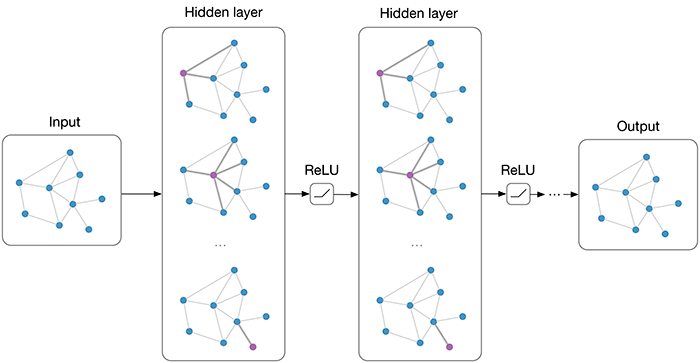
\includegraphics[width=0.8\textwidth]{images/20_material_methods/model.png}
    \caption{Modell für die Graphenklassifizierung (Quelle: \cite{kipf_semi-supervised_2017})}
    \label{fig:gcn_model}
\end{figure}

\newpage
\subsection{Unterschied von Graph-Embedding und Graph-Kernels}

Graph-Kernel-basierte Ansätze zersetzen einen Graphen in eine Menge von Subgraphen, Graphlets \cite{shervashidze_efficient_2009} oder Weisfeiler-Lehman-Kernels genannt \cite{shervashidze_weisfeiler-lehman_nodate}.
Diese Ansätze werden bisher verwendet, um die Ähnlichkeiten zwischen Graphen zu berechnen.
Beim Zersetzen von Graphen in Graph-Kernels geht es darum, möglichst viele Informationen auf ihre zentralen Merkmale zu reduzieren.
Diese Informationen werden dann in einem Vektor zusammengefasst und können mit anderen Vektoren verglichen werden.

Graph-Embedding ist ein Ansatz, welcher in den Graph Neural Networks verwendet wird. Der Ursprung geht auf William Hamilton und das Thema \enquote{Representation Learning} von Graphen zurück \cite{hamilton_inductive_2018}.
Die Aggregationsfunktion $ \phi $ ist ein Graph Neural Network, welches die Eigenschaften der Knoten in einen Vektor transformiert \cite{xu_how_2019}.
Mit der \textsc{ReadOut}-Funktion $ \rho $ werden die einzelnen Vektoren dann via Sum-Pooling zusammengefasst, um Graph-Embedding zu erhalten \cite{nguyen_universal_2022}.

\begin{figure}[H]
    \centering
    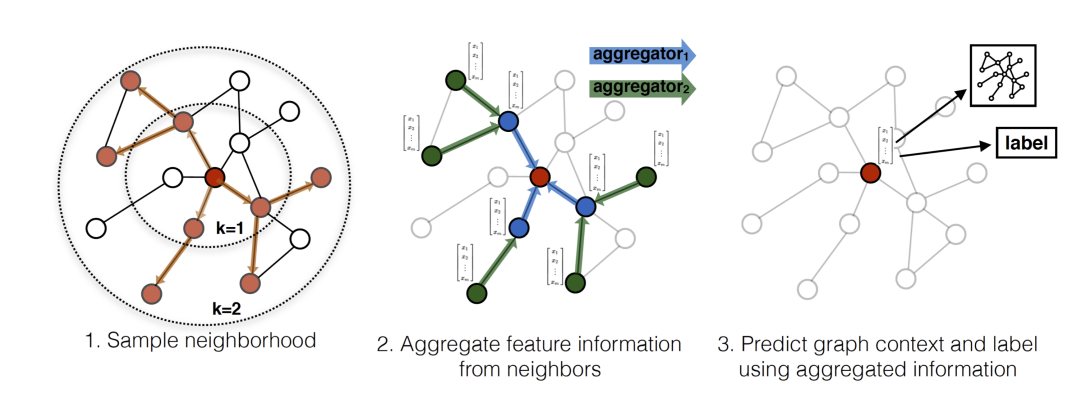
\includegraphics[width=9cm]{images/20_material_methods/graph_representation_learning.png}
    \caption{Sample- und Aggregation-Ansatz visualisiert (Quelle: Hamilton \cite{hamilton_inductive_2018})}
    \label{fig:graph_representation_learning}
\end{figure}
